
\documentclass[10pt]{beamer} 
\usetheme[pageofpages=of,% String used between the current page and the
          % total page count.
          alternativetitlepage=true,% Use the fancy title page.
          %titlepagelogo=coca,% Logo for the first page.
          titleline=true
          ]{Torino}
%\usetheme{Frankfurt}
\usecolortheme{chameleon}

\usepackage{graphicx,hyperref,url}
\usepackage[utf8]{inputenc}
\usepackage[T1]{fontenc}
\usepackage[portuges,brazilian]{babel}
%%%\usepackage{wrapfig}
\usepackage{caption}
\usepackage{subfigure}
%\usepackage{subcaption}
\usepackage{latexsym}
\usepackage{amssymb, amsmath}
\usepackage{multicol}
\usepackage{pifont}%,bbding}%%,dingbat} %%% ver manual de simbolos
\usepackage[final]{listings}
\usepackage{comment}


\definecolor{azulclaro}{rgb}{0.9,0.9,0.9}
\definecolor{mygreen}{rgb}{0,0.6,0}
\definecolor{mygray}{rgb}{0.5,0.5,0.5}
\definecolor{mymauve}{rgb}{0.58,0,0.82}
\definecolor{darkgray}{rgb}{.4,.4,.4}
\definecolor{purple}{rgb}{0.65, 0.12, 0.82}

\newcommand{\minizinc}{MiniZinc}

\lstset{ 
  %  label={pgm_ex01},
    backgroundcolor=\color{azulclaro}, 
    language=erlang, %%Miranda,%%Perl,%%%Python, %%Mercury,
    showstringspaces=false,
    basicstyle=\bf\scriptsize\ttfamily,
%%      basicstyle= \footnotesize %%% TESTAR
%%      keywordstyle=\bfseries\color{green!40!black},
    keywordstyle=\textbf{\color{mygreen}}, 
    otherkeywords={*, \%, array, constraint, solve, output,  show, "/\", satisfy, set, of, if, then, elseif, float, search},
%%  keywordstyle=\color{blue},       % keyword style
%%    commentstyle=\itshape\color{purple!40!black},
      commentstyle=\color{orange},    % comment style
      identifierstyle=\color{blue},
      stringstyle=\color{orange},
      stringstyle=\color{mymauve},
      numbers=left,  % where to put the line-numbers; possible values are (none, left, right)
      numbersep=5pt,   % how far the line-numbers are from the code
      numberstyle=\tiny\color{magenta},
      keepspaces=true      
    % %caption={LEGENDA no source PASCAL ficou OK},
}


\graphicspath{{/home/ccs/Dropbox/figs_genericas/}{figuras/}{/home/ccs/Dropbox/CCS/picat}}
\DeclareGraphicsExtensions{.pdf,.png,.jpg}
%Global Background must be put in preamble
%\usebackgroundtemplate{\includegraphics[width=\paperwidth]{amarelinho.pdf}}
%%% \begin{frame}[allowframebreaks=0.8]

% The log drawn in the upper right corner.

%\logo{\centering
%\includegraphics[height=0.050\paperheight]{figuras/logo_SBPO_Peixe.png}
%%\hspace{9.6cm}
%\includegraphics[height=0.027\paperheight]{figuras/logo_udesc_horizontal.jpg}


%%%%%%%%%%%%%%%%%%%%%%%%%%%%%%%%%%%%%%%%%%%%%%%%%%%%%%%%%%%%%%%%%%%%%


\title[Picat]{\fontsize{20}{30}\selectfont \textcolor{black}{Explicações em Figuras -- ALP}}

\author[]{Claudio Cesar de Sá\\
     {\small \url{claudio.sa@udesc.br}}}

\institute[UDESC]{
    Departamento de Ci\^encia da Computa\c{c}\~ao \\
    Centro de Ci\^encias e Tecnol\'ogias\\
   Universidade do Estado de Santa Catarina}

%%%%%%%%%%%%%%%%%%%%%%%%%%%%%%%%%%%%%%%%%%%%%%%%%%%%%%%%%%%%%%%%%%%%%

\begin{document}

\begin{frame}
    \titlepage
\end{frame}

%%%%%%%%%%%%%%%%%%%%%%%%%%%%%%%%%%%%%%%%%%%%%%%%%%%%%%%%%%%%%%%%%%%%%

%\begin{frame} [allowframebreaks=0.8]
%\frametitle{Sumário}
%\tableofcontents
%\end{frame}

%%%%%%%%%%%%%%%%%%%%%%%%%%%%%%%%%%%%%%%%%%%%%%%%%%%%%%%%%%%%%%%%%%%%%

\begin{frame}[fragile]

\frametitle{Os primeiros computadores}

\begin{figure}[!ht]
\centering
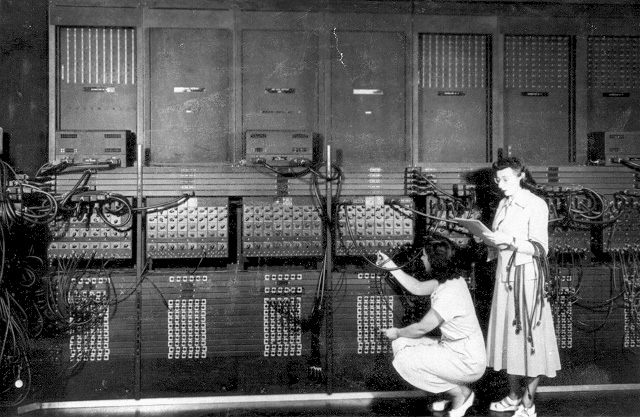
\includegraphics[height =.65\textheight,width=.8\textwidth]
{figuras/antigo_computador.jpg}
%%%\caption{Agente situado versus a visão clássica de sistemas inteligentes}
%\label{ag_01}
\end{figure}

\end{frame}



%-----------------------------------------------------------------------------
\begin{frame}[fragile]

\frametitle{Computador digital -- veja a fita em papel}

\begin{figure}[!ht]
\centering
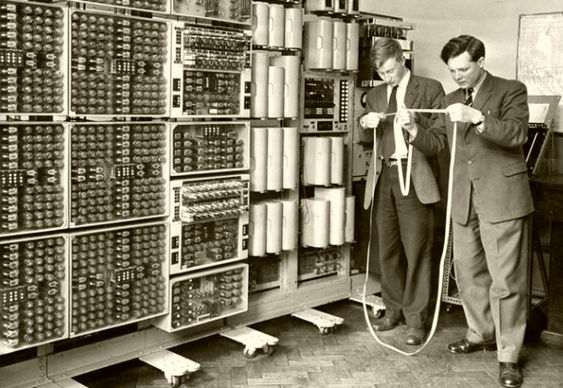
\includegraphics[height =.65\textheight,width=.8\textwidth]
{figuras/computador_digital.jpg}
%%%\caption{Agente situado versus a visão clássica de sistemas inteligentes}
%\label{ag_01}
\end{figure}

\end{frame}
%-----------------------------------------------------------------------------






%-----------------------------------------------------------------------------
\begin{frame}[fragile]

\frametitle{A fita perfurada = codificada}

\begin{figure}[!ht]
\centering
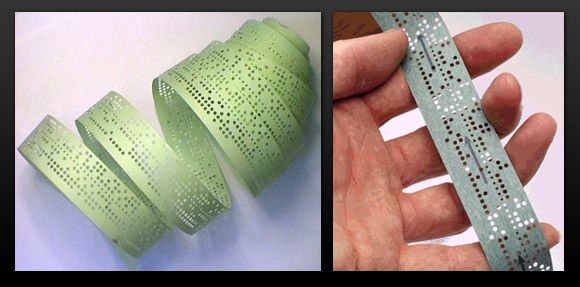
\includegraphics[height =.65\textheight,width=.8\textwidth]
{figuras/fita_perfurada.jpg}
%%%\caption{Agente situado versus a visão clássica de sistemas inteligentes}
%\label{ag_01}
\end{figure}

\end{frame}
%-----------------------------------------------------------------------------



%-----------------------------------------------------------------------------
\begin{frame}[fragile]

\frametitle{Troque \textit{furos} por \textbf{0} e \textit{espaços} por \textbf{1} e bem-vindo ao mundo digital!}

\begin{figure}[!ht]
\centering
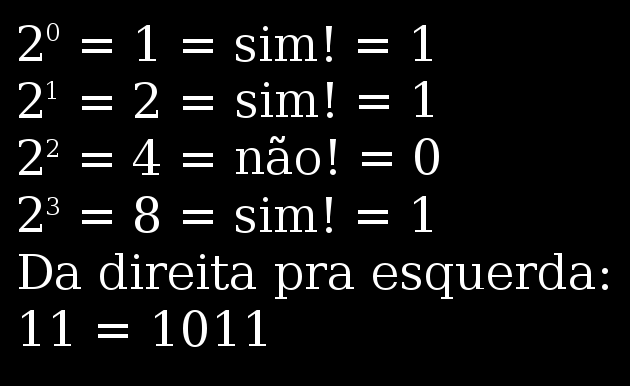
\includegraphics[height =.65\textheight,width=.8\textwidth]
{figuras/computador_internamente.jpg}
%%%\caption{Agente situado versus a visão clássica de sistemas inteligentes}
%\label{ag_01}
\end{figure}

\end{frame}
%-----------------------------------------------------------------------------

%-----------------------------------------------------------------------------
\begin{frame}[fragile]

\frametitle{Melhorando a leitura dos \textbf{0's} e \textbf{1's} $\rightarrow$ sistemas de codificação}

\begin{figure}[!ht]
\centering
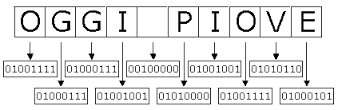
\includegraphics[height =.4\textheight,width=.7\textwidth]
{figuras/bin_codifica_ASCII.png}
%%%\caption{Agente situado versus a visão clássica de sistemas inteligentes}
%\label{ag_01}
\end{figure}

\end{frame}
%-----------------------------------------------------------------------------


%-----------------------------------------------------------------------------
\begin{frame}[fragile]

\frametitle{Internamente ao processador temos algo \textit{análogo} a:}

\begin{figure}[!ht]
\centering
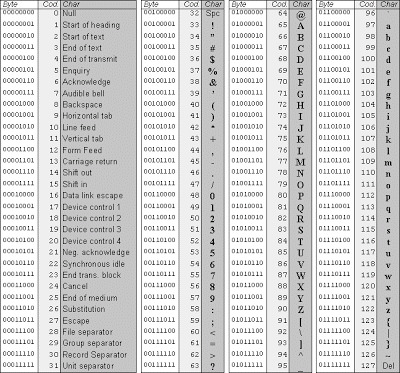
\includegraphics[height =.6\textheight,width=.7\textwidth]
{figuras/instrucoes_CPU.jpg}
\caption{Acreditem ... há sequências binárias, decimais e mnêmonicos!}
%\label{ag_01}
\end{figure}

\end{frame}
%-----------------------------------------------------------------------------


%-----------------------------------------------------------------------------
\begin{frame}[fragile]

\frametitle{Logo, apenas binários nas memórias ...}

\begin{figure}[!ht]
\centering

\includegraphics[height =.5\textheight,width=.4\textwidth]
{figuras/binarios_memoria.jpg}
%%%\caption{Agente situado versus a visão clássica de sistemas inteligentes}
%\label{ag_01}
\end{figure}

\end{frame}
%-----------------------------------------------------------------------------


%-----------------------------------------------------------------------------
\begin{frame}[fragile]

\frametitle{Relembrando um PC internamente $\equiv $ computador}

\begin{figure}[!ht]
\centering
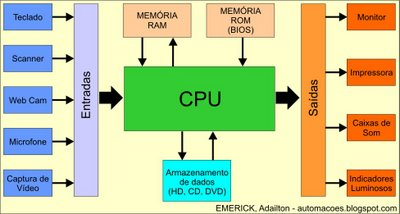
\includegraphics[height =.5\textheight,width=.7\textwidth]
{figuras/estrutura-PC.jpg}
%%%\caption{Agente situado versus a visão clássica de sistemas inteligentes}
%\label{ag_01}
\end{figure}

\end{frame}
%-----------------------------------------------------------------------------


%-----------------------------------------------------------------------------
\begin{frame}[fragile]

\frametitle{Sistema decimal (compreensível para nós) logo: decimal $\Leftrightarrow$ binário}

\begin{figure}[!ht]
\centering
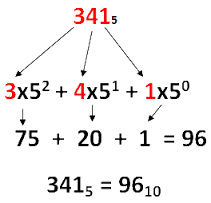
\includegraphics[height =.5\textheight,width=.6\textwidth]
{figuras/sistema_decimal.png}
%%%\caption{Agente situado versus a visão clássica de sistemas inteligentes}
%\label{ag_01}
\end{figure}

\end{frame}
%-----------------------------------------------------------------------------



%-----------------------------------------------------------------------------
\begin{frame}[fragile]

\frametitle{Binário para decimal}

\begin{figure}[!ht]
\centering
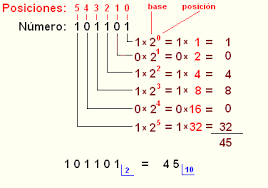
\includegraphics[height =.65\textheight,width=.8\textwidth]
{figuras/binario_decimal.png}
%%%\caption{Agente situado versus a visão clássica de sistemas inteligentes}
%\label{ag_01}
\end{figure}

\end{frame}
%-----------------------------------------------------------------------------



%-----------------------------------------------------------------------------
\begin{frame}[fragile]

\frametitle{Decimal para Binário}

\begin{figure}[!ht]
\centering
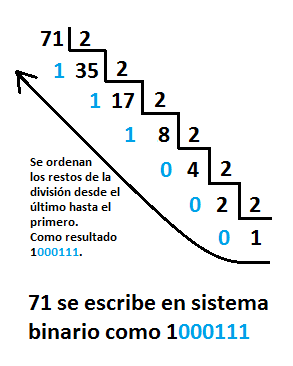
\includegraphics[height =.65\textheight,width=.8\textwidth]
{figuras/decimal_binario.png}
%%%\caption{Agente situado versus a visão clássica de sistemas inteligentes}
%\label{ag_01}
\end{figure}

\end{frame}
%-----------------------------------------------------------------------------

%-----------------------------------------------------------------------------
\begin{frame}[fragile]

\frametitle{O que vamos fazer no curso (\textcolor{red}{\textbf{gravem esta figura}}):}

\begin{figure}[!ht]
\centering
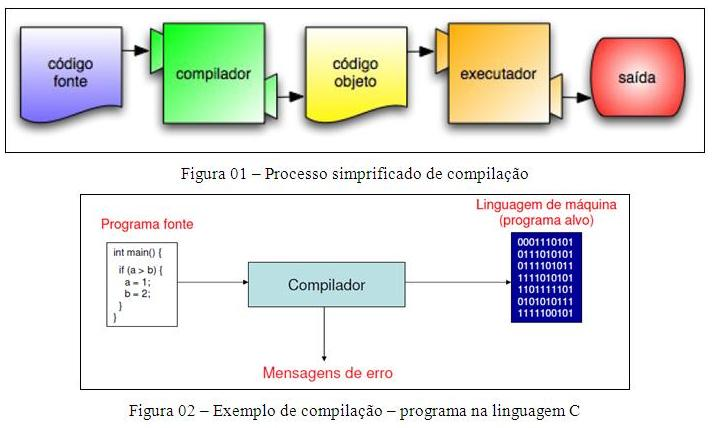
\includegraphics[height =.65\textheight,width=.8\textwidth]
{figuras/compilacao_01.jpg}
%%%\caption{Agente situado versus a visão clássica de sistemas inteligentes}
%\label{ag_01}
\end{figure}

\end{frame}
%-----------------------------------------------------------------------------


%-----------------------------------------------------------------------------
\begin{frame}[fragile]

\frametitle{Válido para qualquer Sistema Operacional (SO):}

\begin{figure}[!ht]
\centering
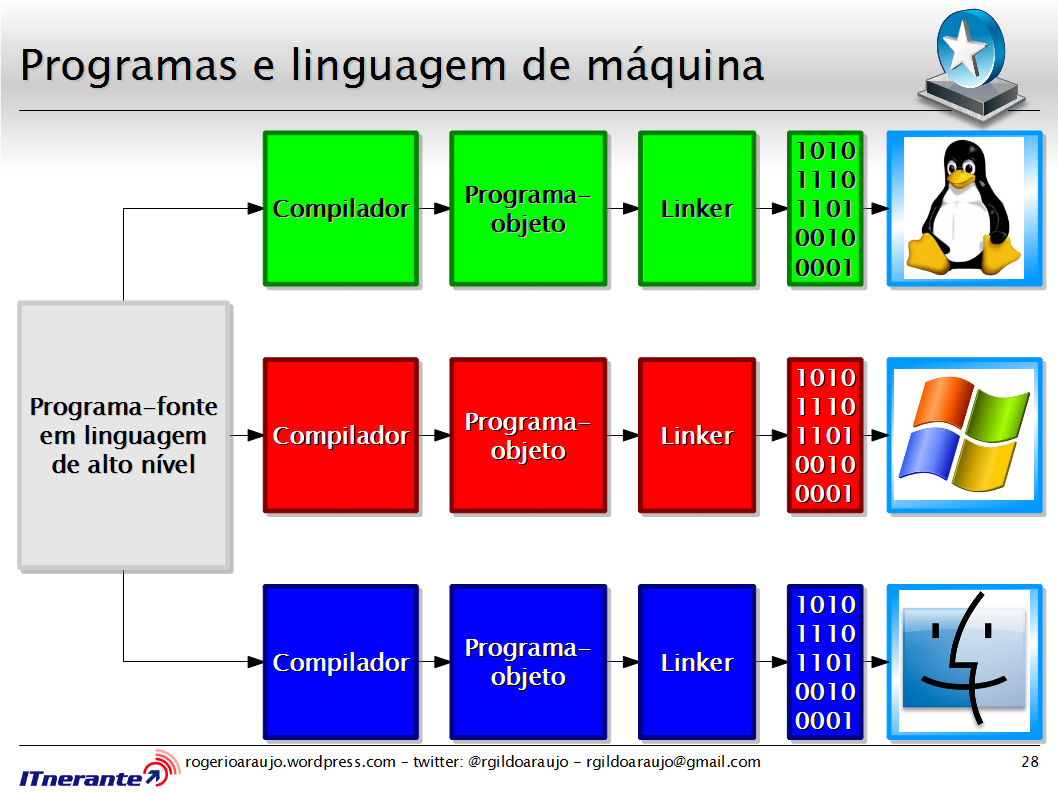
\includegraphics[height =.65\textheight,width=.8\textwidth]
{figuras/compilacao_02.png}
%%%\caption{Agente situado versus a visão clássica de sistemas inteligentes}
%\label{ag_01}
\end{figure}

\end{frame}
%-----------------------------------------------------------------------------

%-----------------------------------------------------------------------------
\begin{frame}[fragile]

\frametitle{Pois vamos fazer aplicações (fontes e executáveis) usuários!}

\begin{figure}[!ht]
\centering
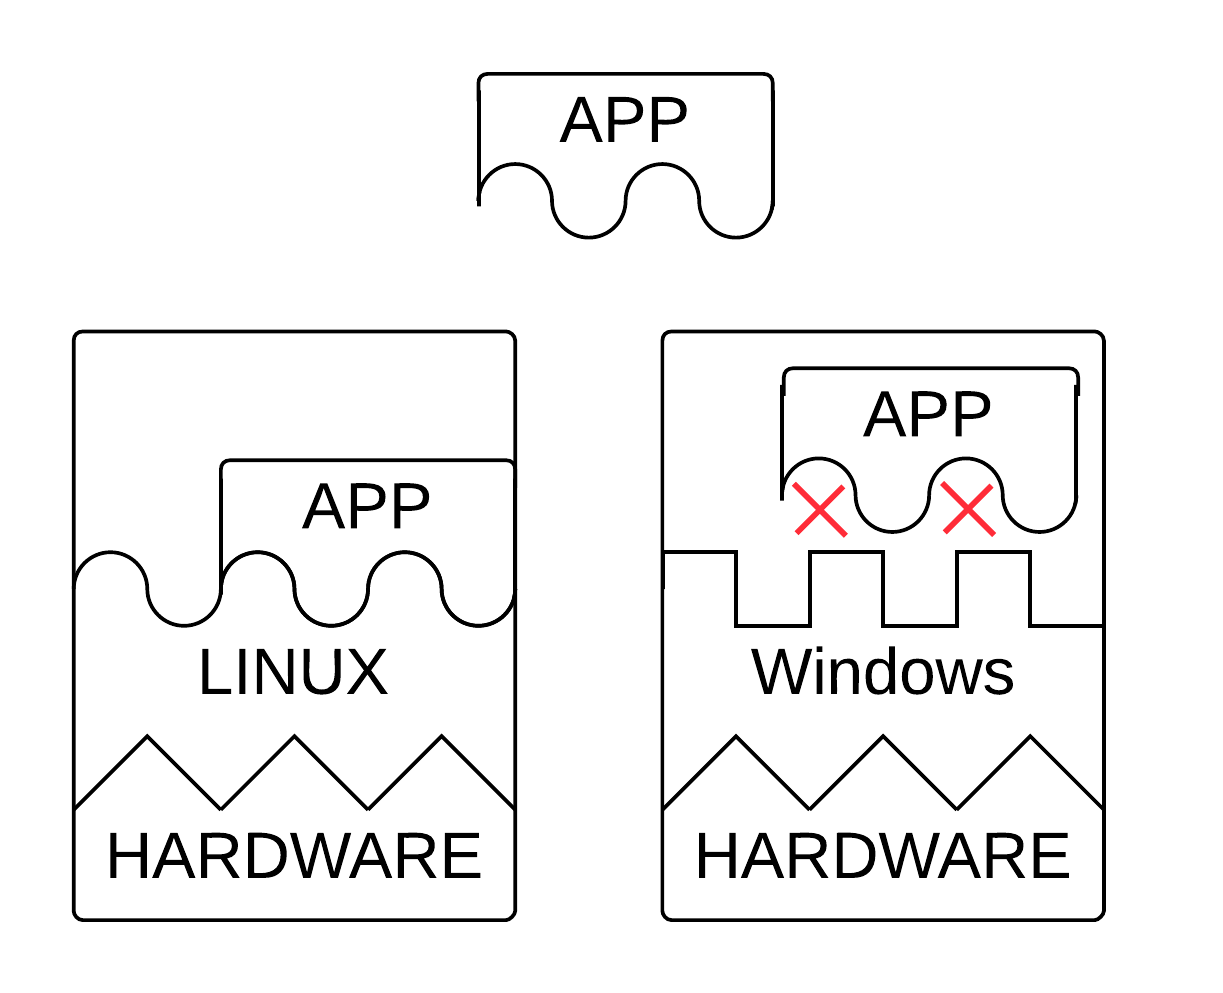
\includegraphics[height =.65\textheight,width=.8\textwidth]
{figuras/aplicacao_usuario.png}
%%%\caption{Agente situado versus a visão clássica de sistemas inteligentes}
%\label{ag_01}
\end{figure}

\end{frame}
%-----------------------------------------------------------------------------

%-----------------------------------------------------------------------------
\begin{frame}[fragile]

\frametitle{Programas aos usuários!}

\begin{figure}[!ht]
\centering
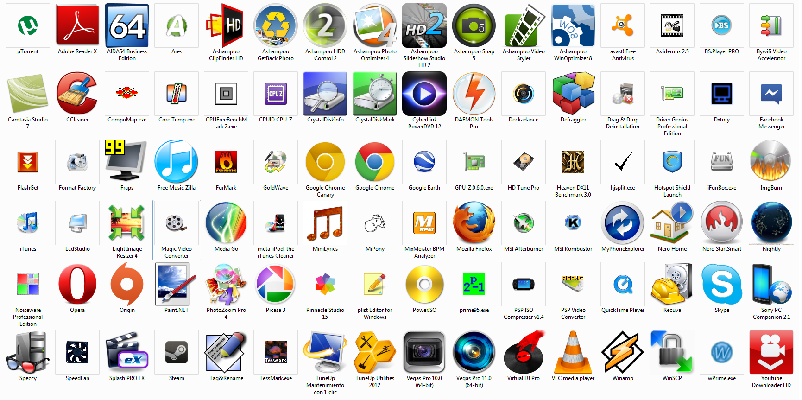
\includegraphics[height =.65\textheight,width=.8\textwidth]
{figuras/programas.png}
%%%\caption{Agente situado versus a visão clássica de sistemas inteligentes}
%\label{ag_01}
\end{figure}

\end{frame}
%-----------------------------------------------------------------------------
%-----------------------------------------------------------------------------
\begin{frame}[fragile]

\frametitle{Epílogo}

\begin{figure}[!ht]
\centering
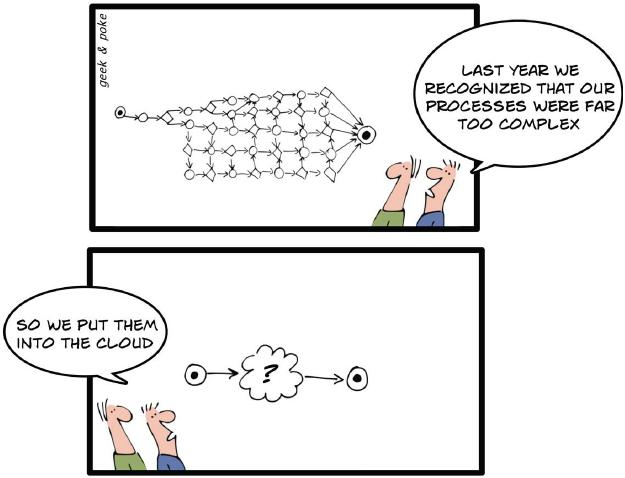
\includegraphics[height =.65\textheight,width=.8\textwidth]
{figuras/Cloud-Computing-Made-Easy.jpg}
%%%\caption{Agente situado versus a visão clássica de sistemas inteligentes}
%\label{ag_01}
\end{figure}

\end{frame}
%-----------------------------------------------------------------------------



%%%%%%%%%%%%%%%%%%%%%%%%%%%%%%%%%%%%%%%%%%%%%%%%%%%%%%%%%%%%%%%%%%%%%

\end{document}
